\chapter{Hydrodynamical and sedimentary analysis}
\label{chap:hydroanalysis}
\section{Effect of tides and waves on the water level}
In addition to the study on the effects of sand mining on the river bed, it is as important to look at the effects of water on the river banks.

\subsection{Tides, waves and currents}
Relevant to this project, the two situations that contribute to this problem are the elevation of the water level due to the high astronomical tide, and the elevation of the water level/current due to the ship waves.

\subsubsection{Astronomical tides}

The tides are the rise and fall of the water level, in particular the sea level, due to the gravitational force of the moon\autocite{usdepartmentofcommerceTidesCurrents}. As said, the tidal influence is the strongest in the ocean, pulling away the sea from one side of the globe to the other in function of the position of the moon, as seen in Figure 2.5.
\begin{figure}[H]
    \centering
    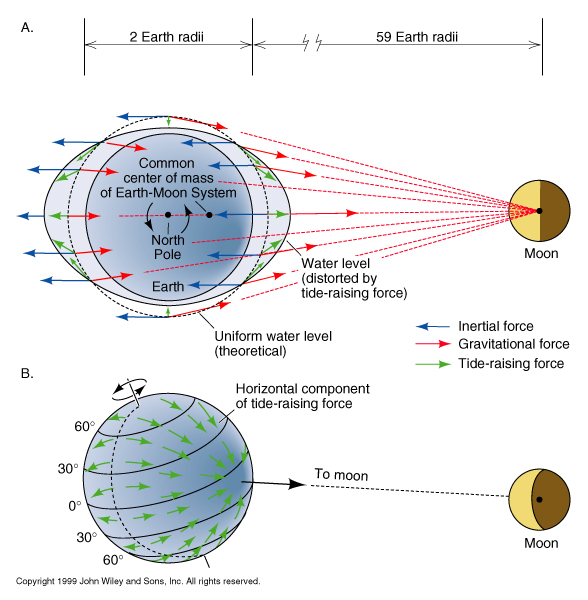
\includegraphics[width=0.5\linewidth]{figures/ch2/astronomical.jpg}
    \caption{Tidal movement due to gravitational force}
    \label{fig:placeholder}
\end{figure}
This gravitational force can also apply to rivers, as long as they are part of, or near a substantial quantity of water mass. Since the region of interest the  Rio Paraná Guazú and Ibicuy are quite near the delta of the Paraná and the river mouth, it is expected to be of significance for the data analysis. This will be treated in section \ref{sec 5.2 Hydrodynamic data}.

\subsubsection{Waves}

The gravitational force not only yields a change in water level, but is also responsible for tidal waves. These are induced by the gravitational pull, in the direction of the moving current. 
In addition to that, there are also wind waves. These are produced by a striking distance called the fetch, where the wind blows on the surface of the water, gathering energy which translates into a wave. In order to find the significant wave height of this situation, one takes a sample of wave heights from buoys and takes the average of the three highest waves. (formula necessary??)

Given the fact that the river is not straight, the fetch or striking distance is usually quite short, as seen in Figure \ref{Figure 1.1}. This means that the impact of the wind waves is probably quite small. This subject will also be treated in section \ref{sec 5.2 Hydrodynamic data}.

The last part of the waves that will be treated in this subsection are the ship waves. These are created when a ship passes by and pushes away the water to make way for the boat to go forward. This situation initiates three types of waves, primary, secondary, and propeller wash waves\autocite{}, as seen in Figure 2.6 below.
\begin{figure}[H]
    \centering
    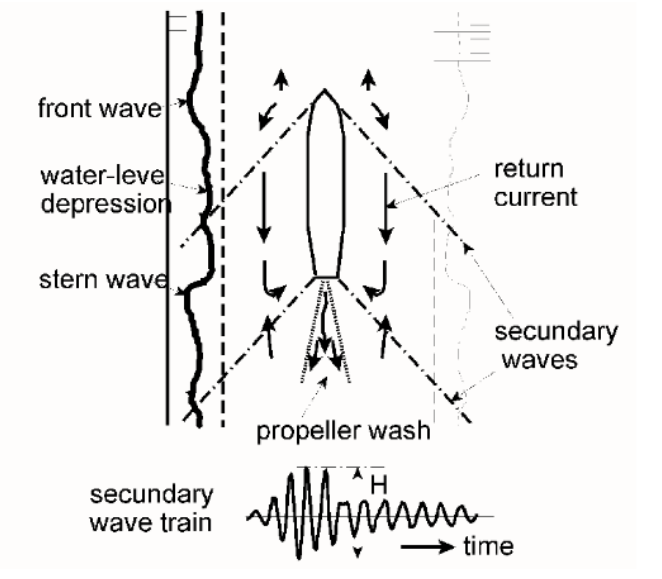
\includegraphics[width=0.5\linewidth]{figures/ch2/afbeelding.png}
    \caption{Ship Waves}
    \label{fig:placeholder}
\end{figure}
The impact of the secondary wave is the most promiscuous, as one can tell from the frequency plot underneath the sketch.



\subsubsection{Correlated currents}

Due to changes in water level as well as supplementary waves, a change in current applies. Using the standard values of the Netherlands and the given facts about the size of the ships circulating and the currents in the Rio Paraná Guazú, one could assume the wave height and current amplitudes for our case. This can be reflected once the field measures are known, in a later section \ref{Section 5}.
The table of the referencing values are as follows:

\begin{table}[H]
    \centering
    \caption{Standard values for wave heights and currents in the Netherlands (Data from CUR 197 ``Breuksteen in de praktijk'').}
    \label{tab:standard_values}
    \begin{tabular}{lcccc}
        \toprule
        \textbf{Location} & \multicolumn{2}{c}{\textbf{Wave heights (m)}} & \multicolumn{2}{c}{\textbf{Currents (m/s)}} \\
        \cmidrule(lr){2-3} \cmidrule(l){4-5}
        & \textbf{Wind waves} & \textbf{Ship waves} & \textbf{Natural current} & \textbf{Return current} \\
        \midrule
        Lakes          & 0.25 -- 1.00  & 0.10 -- 0.50  & 0.1 -- 0.5  & 0.1 -- 0.25 \\
        Canals         & 0.10 -- 0.25  & 0.25 -- 0.75  & 0.5 -- 1.0  & 0.5 -- 1.0  \\
        Rivers         & 0.25 -- 1.00  & 0.25 -- 0.75  & 1.0 -- 2.0  & 0.5 -- 1.0  \\
        Small waters   & 0.10 -- 0.20  & n.a.          & 0.2 -- 1.0  & n.a.       \\
        \bottomrule
    \end{tabular}
\end{table}


Understandably, the relevant row for this project is the 'River' category. Hinting to the fact that big ships are usually present in the channel, one might take values towards the upper boundary of the table.


\subsection{Effect on the river bed}

There are several ways how the water could have a negative impact on the river bank. In theory the river bank failure may be caused by house placement, water saturation, weight on the river bank, vegetation, and/or tectonic activity, but most of them due to the rise of the water level. The reason behind this is that the river bank is naturally eroded when the water exerts a force on it.
The river bank is divided in three parts: the toe, the bank and the overbank zone. The toe of the bank is the most susceptible to erosion when in contact with high water levels, which can be seen in the Figure 2.7 below \autocite{australiaRiverbankCollapse}.

\begin{figure}[H]
    \centering
    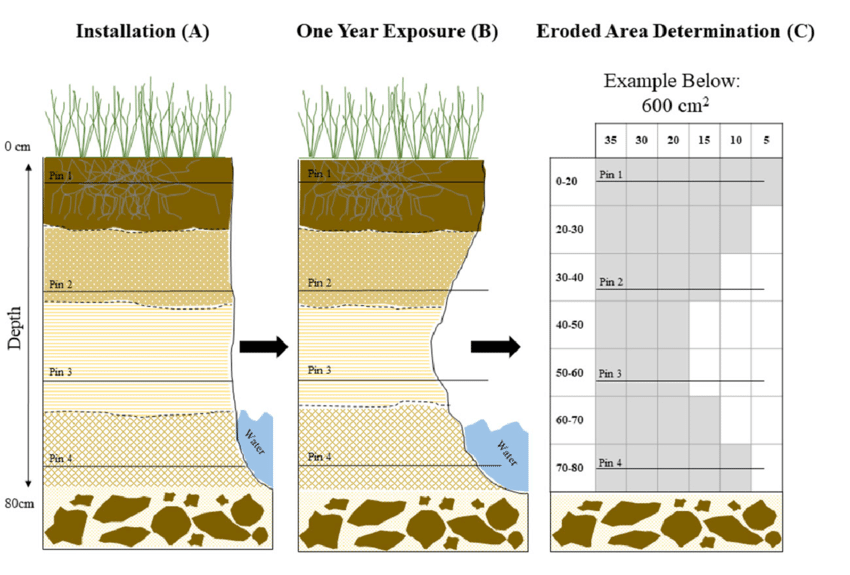
\includegraphics[width=0.5\linewidth]{figures/ch2/Erosion.png}
    \caption{Effect of Water on Bank after One Year}
    \label{fig:placeholder}
\end{figure}

When the combination of water level with a strong current is highest, the bank zone is affected by the tidal currents or waves. This is because, as seen in the Figure 7.2, water erodes the layer of the bank where the extra water level pushes, creating a dent inside the soil layer.
Consequently, after some time the upper overbank area has less and less support underneath, becoming thus unstable and partly falling down. 
Repeating this process takes the river bank further inside the land, increasing the channel width, absorbing the land of the local communities or agricultural fields that live near the river bank.


\section{Hydrodynamic data}
\label{sec 5.2 Hydrodynamic data}
In this section, analysis on the hydrodynamic variables is performed. This includes relations between water elevations, discharge and sediment concentrations - both through data sources and field measurements. Additionally, tidal effects in the study area are considered. 

\subsection{Conversion to water elevation}
A uniform approach is needed to describe water levels and depths of the river. Therefore, these variables will be expressed in terms of a reference level, IGN, which is set by the \textit{Instituto Geográfico Nacional}. It is based on sea level measurements from a tide gauge in Mar del Plata, Buenos Aires province (\cite{ReferenciaVerticalInstituto}). Figure \ref{fig:waterelevationreference} gives an overview of the quantities with respect to an arbitrary measurement station. Here, $d$ is the vertical depth as measured by the ADCP or echosounder. Moreover, each station has a specific distance between its local zero reference and the zero IGN level, which is indicated by $l_{station-IGN}$. Next, values for water level and elevations at the bottom of the river should be expressed in terms of IGN level. Therefore, water elevations and depths expressed in elevation are defined as follows:

\begin{equation}
    we_{station} = wl_{station} + l_{station-IGN} ~[m~IGN]
\end{equation}

\begin{equation}
    d_{el} = we_{station}-d ~[m~IGN]
\end{equation}


\begin{figure}[H]
    \centering
    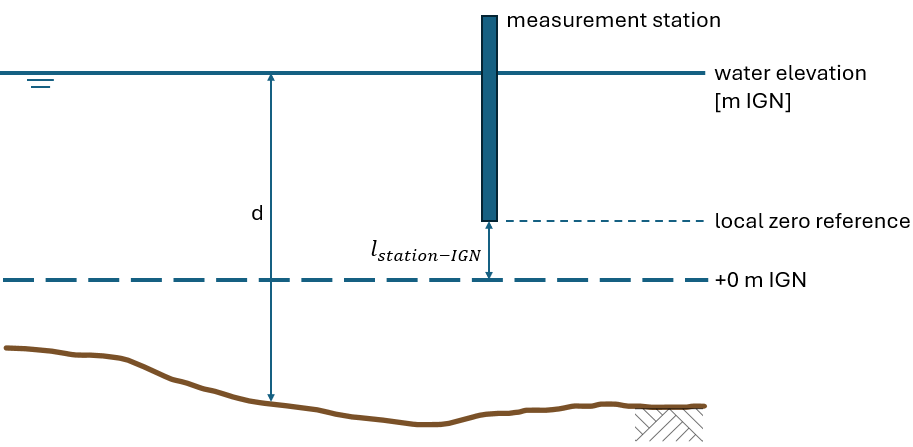
\includegraphics[width=0.75\linewidth]{figures/ch5/waterelevations.png}
    \caption{Water elevation reference}
    \label{fig:waterelevationreference}
\end{figure}

\subsection{Flow partitioning}

At some point in the Lower Paraná, the river splits into two main tributaries, as shown in Figure \ref{fig:flow partition}. To have an approximation for the distribution of discharge between these rivers, the discharge series are given in Figure \ref{fig:discharge_series}. From these plots, it follows that the majority of the discharge flows into the Paraná Guazú. Figure \ref{fig:flow_partition} represents this ratio and plots a linear fit. As there is no significant increase or decrease, the approximation is made that 78\% of the total discharge upstream of the confluence flows into Paraná Guazú. \citeauthor{reMETODOLOGIAPARAGENERACION2009} report that a linearly increasing trend occurs. In this study, more data points are used and therefore the approximation of a constant percentage is assumed sufficient. 

\begin{figure}[h!]
    \centering
    % First subfigure
    \begin{subfigure}[b]{0.48\linewidth}
        \centering
        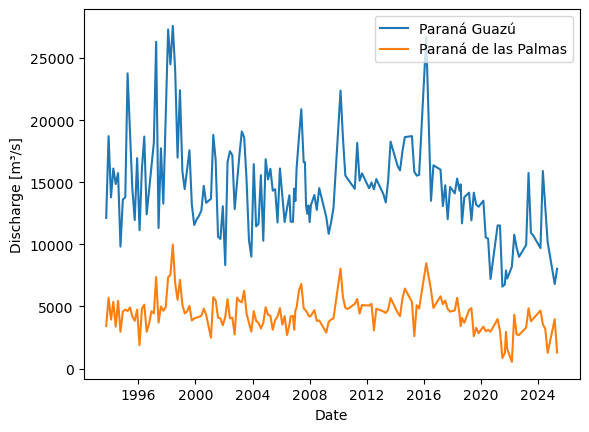
\includegraphics[width=\linewidth]{figures/ch5/discharge series.png}
        \caption{Discharge series obtained from Brazo Largo and Zárate measurement stations}
        \label{fig:discharge_series}
    \end{subfigure}
    \hfill
    % Second subfigure
    \begin{subfigure}[b]{0.48\linewidth}
        \centering
        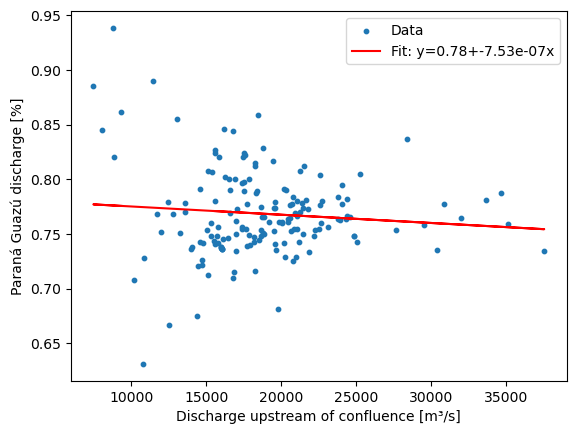
\includegraphics[width=\linewidth]{figures/ch5/flow partition.png}
        \caption{Flow partition, expressed as the share of total flow that streams into Paraná Guazú}
        \label{fig:flow_partition}
    \end{subfigure}
    
    \caption{Comparison of discharge divided between Paraná Guazú and Paraná de las Palmas}
\end{figure}

In order to further study the liquid flows in the Paraná Guazú, it is noted that estimates for the discharge of Río Ibicuy and Río Talabera are needed. These were collected during the fieldwork, as indicated in Figure \ref{fig:measurements day1} and Figure \ref{fig:measurements day2}. In addition, an overview of all cross sections with discharge measurements is given in Figure \ref{fig:cross section domain}. The indexing of the cross sections is made in chronological order based on the fieldwork. Note that at the confluence of the Ibicuy and Paraná Guazú, there is no measurement of the component flowing in from the Paraná Gauzú. However, this can be estimated by the equilibrium of discharges in the confluence. The relevant flow measurements of the different cross sections are summarized in Table \ref{tab:discharges fieldwork}. The bathymetries and velocity profiles that result from the ACDP measurements can be found in Appendix \ref{appendix:fieldwork results}, where the output of the \textit{RiverSurveyor} software is given. Note that of each cross section, only one of the two measured sections is given. 

\begin{table}[H]
    \centering
    \renewcommand{\arraystretch}{1.2} % extra row spacing
    \setlength{\tabcolsep}{8pt}       % extra column spacing
    \begin{tabular}{llccc}
        \toprule
        \textbf{Section} & \textbf{River} & \textbf{Water level [m IGN]} & \textbf{Flow velocity [m/s]} & \textbf{Discharge [$m^3$/s]} \\
        \midrule
        1 & Talabera       &  &  & 4402 \\
        2 & Paraná Guazú   &  &  & 6562 \\
        3 & Paraná Guazú   &  &  & 10748 \\
        4 & Ibicuy         &  &  & 2901 \\
        5 & Paraná Guazú   &  &  & 6758 \\
        \bottomrule
    \end{tabular}
    \caption{Flow properties of fieldwork measurements in different sections}
    \label{tab:discharges fieldwork}
\end{table}


\begin{figure}[H]
    \centering
    \includegraphics[width=0.75\linewidth]{figures/ch5/balance domain.png}
    \caption{Overview of cross sections with discharge measurements}
    \label{fig:cross section domain}
\end{figure}



\subsection{Fluvial forcing}
This section describes the discharge quantities throughout the study area and relates them to water level data. Traditionally, stage-discharge relations are described by rating curves that describe power-law dependencies between variables. This can be written in the following form, with $Q$ the discharge and $h$ the water level or stage:

\begin{equation}
\label{eq:powerlaw}
    Q = a \cdot h^b
\end{equation}

In the expression above, $a$ is a constant and $b$ an index exponent. \textbf{Schmidt and Yen} note several limitations related to these rating curves. For example, discharge measurements typically scatter and therefore do not show a unique relation with the stage. Also, the underlying physics of the open channel are not captured in the rating. Nevertheless, the relation as given in Equation \ref{eq:powerlaw} is used to roughly approximate dependencies between the variables. First, the values in the dataset are log-transformed, after which $R^2$-values are calculated based on a linear fit on the logarithmic values. This procedure is applied to the data of all measurement stations as described in Section \ref{sec:measurementstations}. Figure \ref{fig:correlationmatrices} gives the results for El Colorado and Brazo Largo in the form of correlation matrices. 

\begin{figure}[h!]
    \centering
    % First subfigure
    \begin{subfigure}[b]{0.48\linewidth}
        \centering
        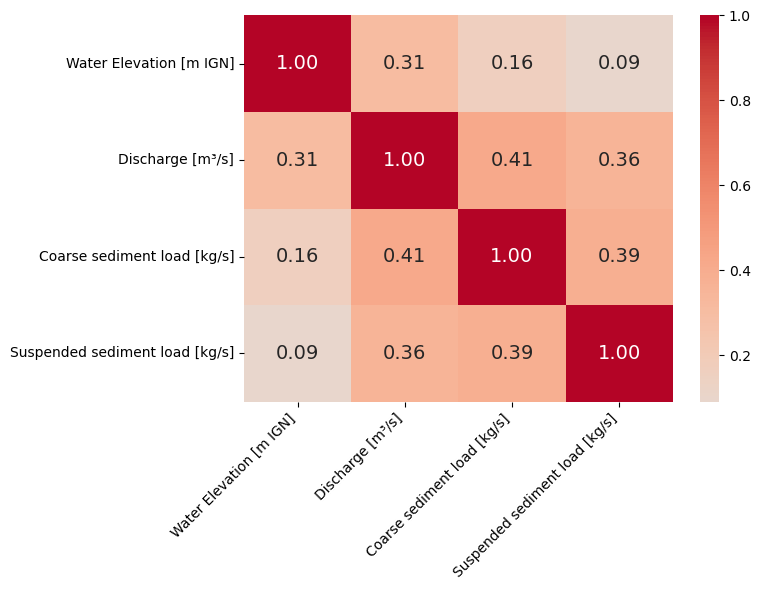
\includegraphics[width=\linewidth]{figures/ch5/logcorrelations Brazo Largo.png}
        \caption{Correlation matrix of log-transformed data in Brazo Largo}
        \label{fig:logcorrelation brazo}
    \end{subfigure}
    \hfill
    % Second subfigure
    \begin{subfigure}[b]{0.48\linewidth}
        \centering
        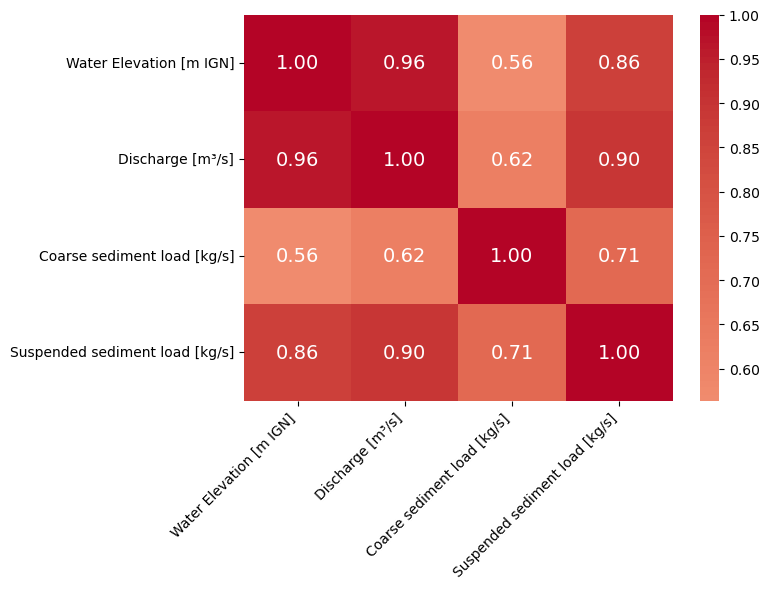
\includegraphics[width=\linewidth]{figures/ch5/logcorrelations Bermejo.png}
        \caption{Correlation matrix of log-transformed data in El Colorado}
        \label{fig:logcorrelation bermejo}
    \end{subfigure}
    
    \caption{Comparison of $R^2$-values at Brazo Largo and El Colorado}
    \label{fig:correlationmatrices}
\end{figure}

The relationship between fluvial discharge and water level at Brazo Largo was initially assumed to follow a power-law, but this yielded a weak correlation with an $R^2$ of 0.261. A linear fit, however, produced a slightly better result, showing a positive trend with an $R^2$ of 0.444 (Figure \ref{fig:waterleveldischarge}).

In contrast, the El Colorado and Túnel Subfluvial stations exhibit a clear power-law dependence. Power-law fits for these stations resulted in higher $R^2$-values of 0.962 and 0.712, respectively, with the El Colorado plot shown in Figure \ref{fig:waterleveldischarge}. Overall, these results suggest that the strength of the water level–discharge relationship decreases as the river flows downstream.

\begin{figure}[h!]
    \centering
    % First subfigure
    \begin{subfigure}[b]{0.48\linewidth}
        \centering
        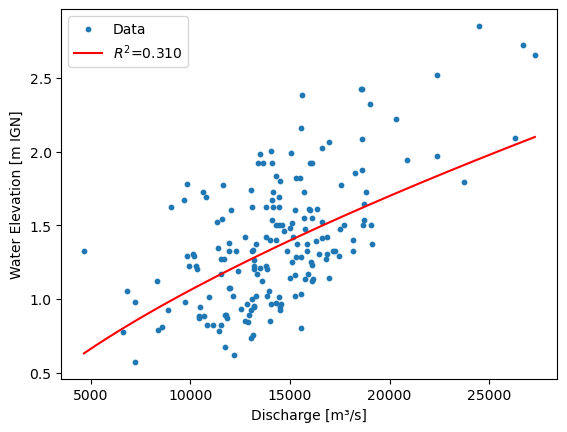
\includegraphics[width=\linewidth]{figures/ch5/wl discharge Brazo Largo.png}
        \label{fig:water level discharge Brazo Largo}
    \hfill
    % Second subfigure
    \end{subfigure}
    \begin{subfigure}[b]{0.48\linewidth}
        \centering
        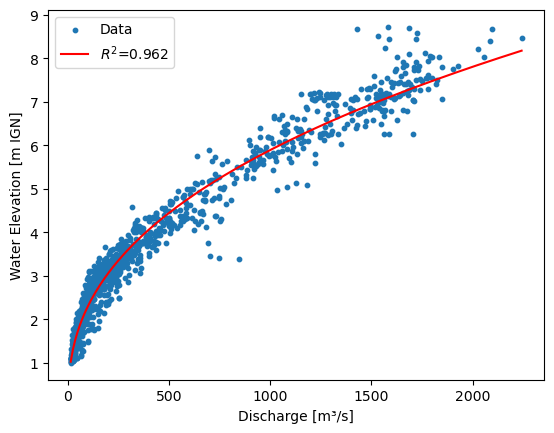
\includegraphics[width=\linewidth]{figures/ch5/wl discharge El Colorado.png}
        \label{fig:water level discharge Colorado}
    \end{subfigure}
    \caption{Water elevation - discharge relationship for two measurement stations}
    \label{fig:waterleveldischarge}
\end{figure}

When extending the analysis to the sediment concentrations, the same trend occurs: in the Bermejo river, fine and course sediment discharges are closely related to large flow events through power-law relations. This behaviour is found to a lesser extent in the lower Paraná, where the correlations are relatively weak. Figure \ref{fig:discharge sediment brazo} shows this relation between sediment concentrations and river discharge for the Brazo Largo station. Overall, a power-law fit seems a good approach to model the relation. The fine sediment concentration is generally higher than the course sediment concentration. In addition, the course sediment concentration increases more significantly for an increasing fluvial discharge. These are general trends, but it has to be stressed that the $R^2$ of both relationships is relatively low.  


\begin{figure}[h!]
    \centering
    % First subfigure
    \begin{subfigure}[b]{0.48\linewidth}
        \centering
        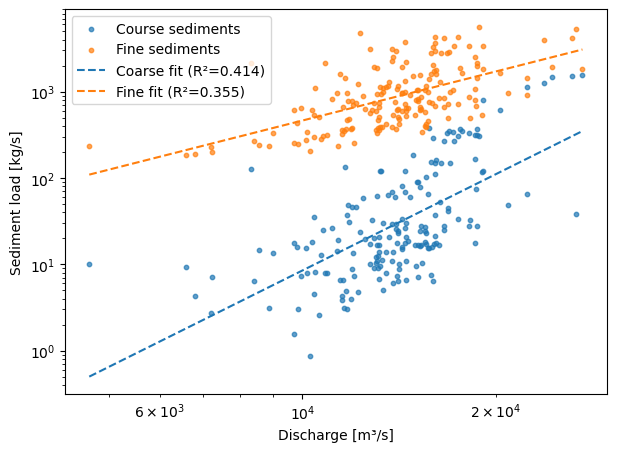
\includegraphics[width=\linewidth]{figures/ch5/discharge sediment brazo largo.png}
        \caption{Fine and course sediment loads in relation to discharge at Brazo Largo}
        \label{fig:discharge sediment brazo}
    \end{subfigure}
    \hfill
    % Second subfigure
    \begin{subfigure}[b]{0.48\linewidth}
        \centering
        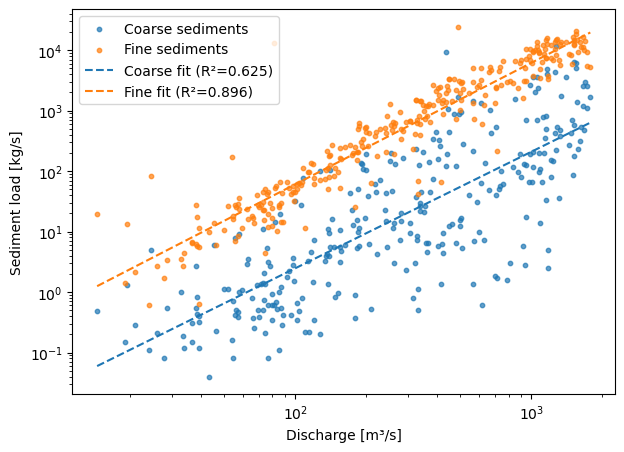
\includegraphics[width=\linewidth]{figures/ch5/discharge sediment bermejo.png}
        \caption{Fine and course sediment concentrations in relation to discharge at Bermejo}
        \label{fig:discharge sediment bermejo}
    \end{subfigure}
    
    \caption{Fine and course sediment loads related to fluvial discharge in two measurement station}
    \label{fig:sediment loads and discharge}
\end{figure}



\subsection{Tidal forcing}
The tidal wave of the Atlantic Ocean influences the hydrodynamics of the lower Paraná delta. As the tidal wave enters the delta ta Río de la Plata, the tide is damped and phased by friction, channel geometry and branching, resulting in a reduced amplitude and an increased in phase delay. Under normal conditions, the influence of the tide on the Paraná River reaches the city of Villa Constitución, which is located 220 km upstream of the river mouth. For storm conditions, the tide can reach the city of Rosario \autocite{balayCAUSESPERIODICITYLARGE1958}. In order to determine the influence of the tide at Brazo Largo, a reference water level at San Fernando is considered. It is assumed that at San Fernando no tidal damping has occurred, therefore the tidal amplitude at Brazo Largo can be determined using the following relation:

\begin{equation}
    A_{\text{Location}} = \alpha \cdot A_{\text{SanFernando}}
\end{equation}

The damping coefficient ($\alpha$) and the tidal delay with respect to San Fernando have been determined by Brok (2022). For Brazo Largo, a damping coefficient of 0.3 and tidal delay of 4 hours were found. These values will be used as reference values when isolating the tide at Brazo Largo. The tidal signal is isolated using hourly water level data for a period of more than 2 years from both Brazo Largo and San Fernando. Table 5.2 shows the tidal constituents  considered and their period.

\begin{table}[h!]
\centering
\caption{Tidal constituents used to reconstruct the tide
\autocite{BRON}.}
\label{tab:constituents}
\begin{tabular}{lccc}
\hline
\textbf{Tidal constituent} & \textbf{Name} & \textbf{Period [h]} \\
\hline
\multicolumn{3}{l}{\textit{Semi-diurnal}} \\
\hspace{1em}Principal lunar & M2 & 12.4206\\
\hspace{1em}Principal solar & S2 & 12.0000 \\
\hspace{1em}Lunar elliptical & N2 & 12.6583\\
\hline
\multicolumn{3}{l}{\textit{Diurnal}} \\
\hspace{1em}Lunar-solar declinational & K1 & 23.9345  \\
\hspace{1em}Principal lunar & O1 & 25.8193  \\
\hline
\multicolumn{3}{l}{\textit{Shallow water constituents}} \\
\hspace{1em}Overtide of M2 (quarter-diurnal) & M4 & 6.2103  \\
\hline
\end{tabular}
\end{table}

- uitleg hoe het getijde bepaald is

The tidal amplitude and phase of each constituent for San Fernando and Brazo Largo are displayed in Table 5.3. Additionally, the damping coefficient ($\alpha$) and the tide delay are calculated for the different constituents and shown in Table 5.3. The calculated amplitudes show that the delta has mixed tidal dynamics  (semidiurnal-diurnal)
dominated by the semi-diurnal M2 constituent with contributions from N2, K1 and O1. The overtide M4 plays a minor role. The damping coefficient is consistent across the constituents ranging from 0.23 to 0.33, inditcating that the use of formula 5.3 is valid. The calculated time delay of 4.5 - 5.5 hours is also in line with the time delay calculated by Brok (2022). The damping coefficient of M4 is different because it is generated locally with nonlinear interactions.

\begin{table}[h!]
\centering
\caption{Amplitude and phase comparison}
\begin{tabular}{lcccccc}
\hline
Constituent & $A_{\text{SF}}$ & $A_{\text{BL}}$ & $\alpha$ & tide delay [hr] & $\phi_{\text{SF}}$ [$^\circ$] & $\phi_{\text{BL}}$ [$^\circ$] \\
\hline
M2 & 0.253 & 0.058 & 0.230 & 4.450 & -0.465 & 1.786 \\
S2 & 0.041 & 0.010 & 0.239 & 5.055 & -2.526 & 0.121 \\
N2 & 0.094 & 0.022 & 0.238 & 4.316 & -0.546 & 1.596 \\
K1 & 0.119 & 0.037 & 0.313 & 5.181 & -2.543 & -1.183 \\
O1 & 0.187 & 0.061 & 0.328 & 5.517 & 2.694 & -2.247 \\
M4 & 0.030 & 0.006 & 0.189 & -1.495 & -2.608 & 2.162 \\
\hline
\end{tabular}
\end{table}

Figure 5.7 shows the water level time series for a period of 7 days compared to the calculated tidal signal at Brazo Largo. From this figure, it can be seen that the measured water level follows the same tidal oscillations. However, the tide does not explain all the variability of the water level; the measured water level also shows large variability caused by discharge and wind. 
\\The influence of the strong non-tidal component is confirmed by Figure 5.8, which shows the water level at Brazo Largo for a period of 2 years. The measured water level fluctuates greatly, reaching +2.0 m and -0.5 m while the tidal component is steady at 0.0 m with an amplitude of 0.17 m. The tidal forcing is relatively small compared to the river and seasonal influences. Tidal forcing is therefore subordinate to other forcings such as discharge.

\begin{figure}[H]
    \centering
    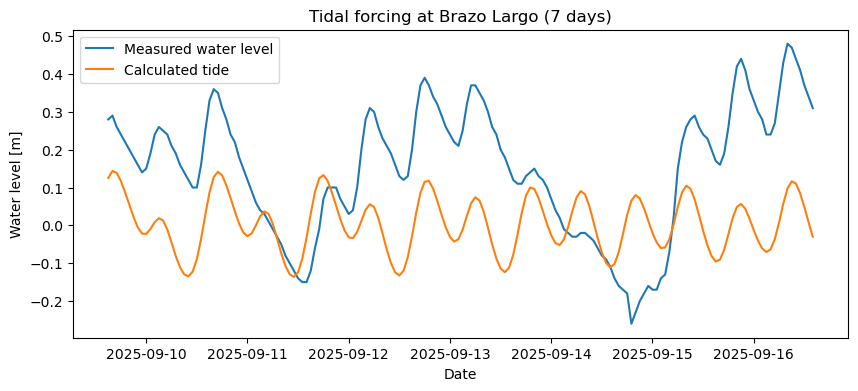
\includegraphics[width=1\linewidth]{figures/ch5/Tide_Brazo_largo.png}
    \caption{Calculated tide at Brazo Largo for a period of 7 days.}
    \label{fig:placeholder}
\end{figure}
\begin{figure}[H]
    \centering
    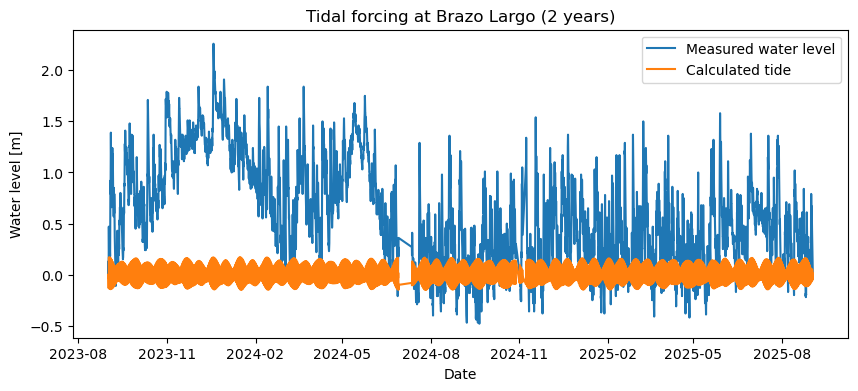
\includegraphics[width=1\linewidth]{figures/ch5/Tide_BL_2y.png}
    \caption{Calculated tide at Brazo Largo for a period of 2 years.}
    \label{fig:placeholder}
\end{figure}

- Waterlevel at Brazo Largo
    (misschien het getijde meenemen?)
\\ - Getijde rond Brazo Largo is berekend aan de hand van waterlevel rond San Fernando. Vergelijk de constituents met die van  het rapport en trek conclusie over invloed getijde.



\section{Sediment transport}




- Bepaal fine sediment-discharge relation bij El Colorado. Reken hiermee door voor het fine sediment concentration bij Brazo Largo

- Bepaal fine sediment concentration op basis van de suspended sediment samples.

- Coarse sediment concentration wordt bepaald met de Engelund-Hansen formule

- Vergelijk dit met de bedload metingen van het veldwerk

- Set up a sediment balance for the area of interest.


- Sediment transport caused by tidal assymetry.


\section{Field work measurements}
Wie doet dit?

\section{Hydrodynamic effects on the River Banks}
\subsection{Aqua Monitor}
In this section the data from the water gains and losses is explained in more detail.
Recalling the whole period of time available \ref{Aqua Monitor Water Changes 1985-2025}, it is clear that the outer side of the river curves experience a water gain (indicated in blue), and the inside sides of the curves lose water (indicated in green). 
The location of the camping 'La Blanqueada' is in the outer side of the curve near Puerto Constanza, as seen in the following Figure \ref{fig:Camping Blanqueada}.

\begin{figure}
    \centering
    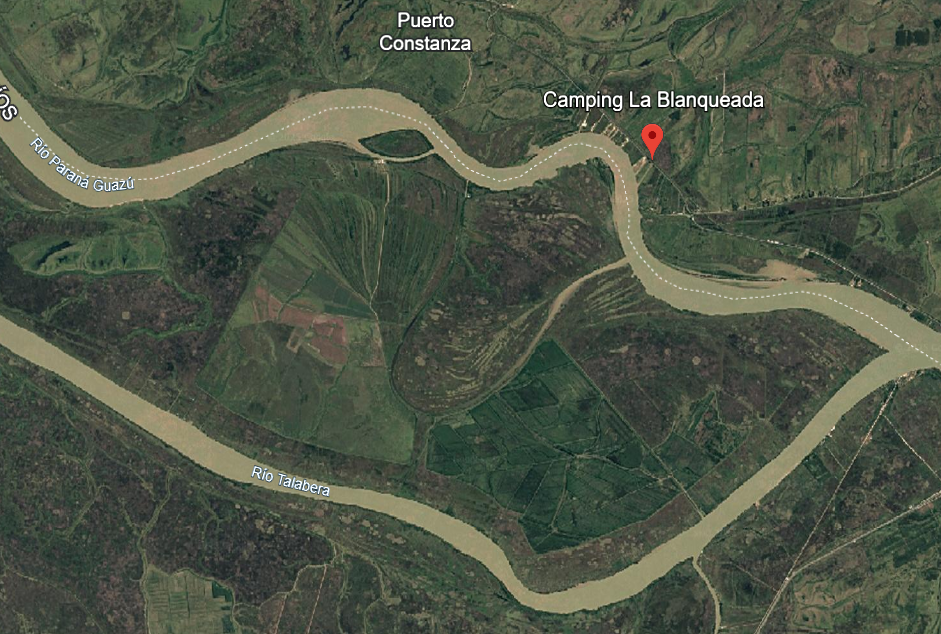
\includegraphics[width=0.5\linewidth]{figures/ch5/Camping Blanqueada.png}
    \caption{Location of the Camping La Blanqueada}
    \label{fig:Camping Blanqueada}
\end{figure}

The camping's location matches with the blue part of the water gain map, indicating that the water quantity around the shore of the camping has increased. 
In order to know if this has always been so, or if the water gains in this precise location have been gradually increasing, several maps with closer intervals have been created. 

There are quite a few comments to be made about the maps. 

First of all, blue and green zones stay consistent throughout the years, but when going into detailed time periods they can differ.

There can be variations in shorter time periods such as the period 2005-2015 which indicated more water gains than losses in the deltas surrounding the region of interest.

Another very interesting thing to note is that the flood of 2016 in the Parana Guazu can also be seen through the help of this map, on a time interval of 2015-2017.

Furthermore, droughts are also illustrated quite well with this software. The perfect example would be the long period of drought in 2022 which led some parts of the Parana to be left for dry, as seen in Figure \ref{fig:Discharge Changes in Brazo Largo}. With the Parana Guazu's significant depths of over 40 meters this was unlikely to happen but still, this change in water quantity did not go unnoticed by the Deltares software. This can be seen on the Figure of 2020-2022.

Other periods of time are more or less stable and have nothing to report.

\begin{figure}[H]
    \centering
    \begin{subfigure}[a]{0.6\textwidth}
        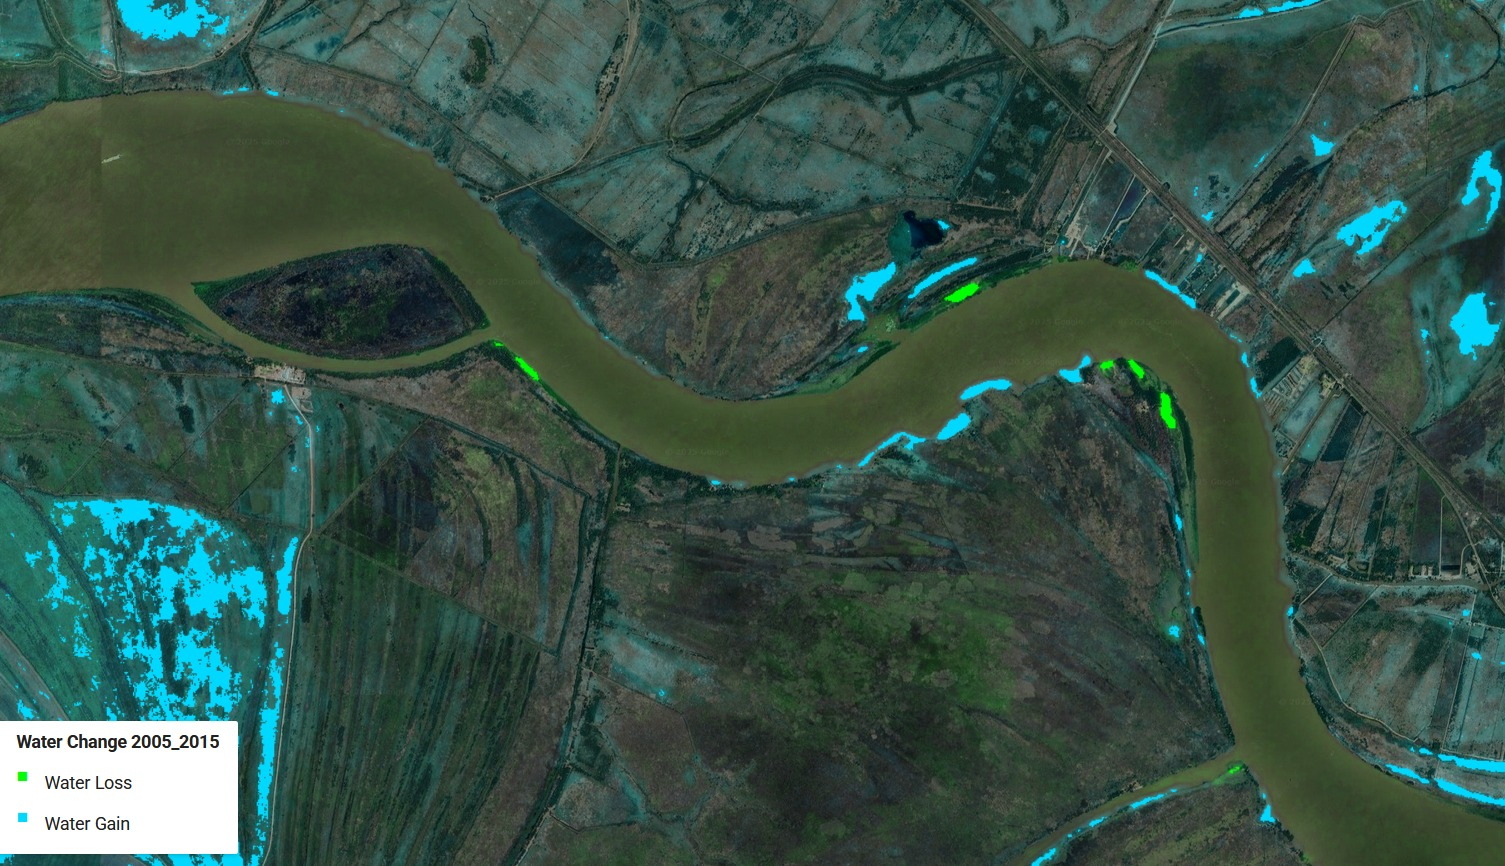
\includegraphics[width=\linewidth, height=5cm]{figures/ch5/2005-2015.jpg}
        \caption{Period 2005-2015}
        \label{fig:sontek}
    \end{subfigure}
\end{figure}

\begin{figure}[H]
    \centering
    \begin{subfigure}[b]{0.6\textwidth}
        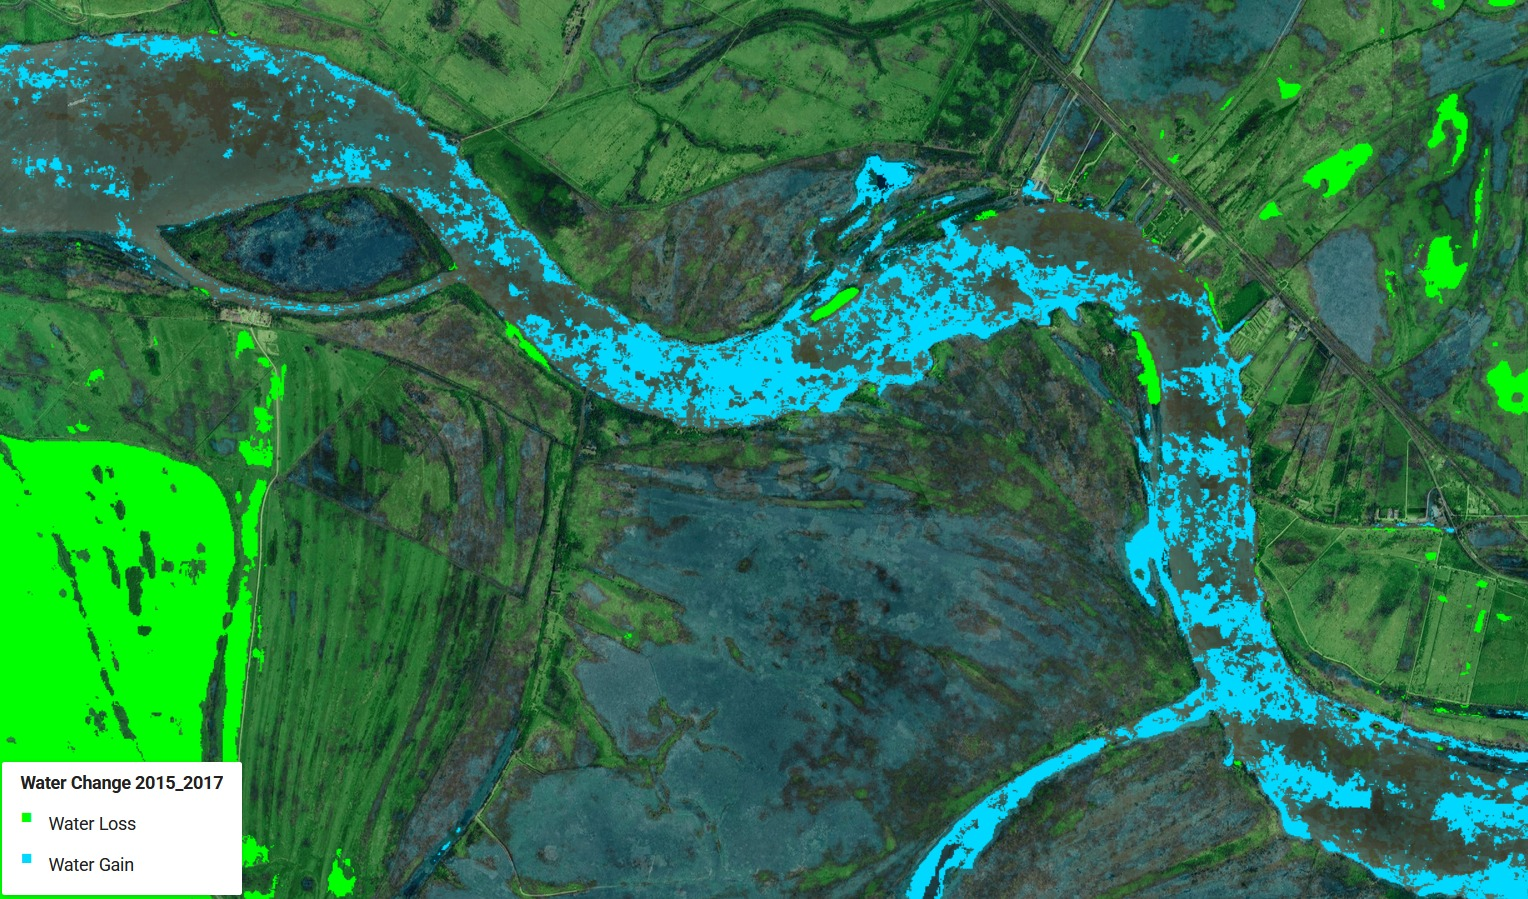
\includegraphics[width=\linewidth, height=5cm]{figures/ch5/2015-2017.jpg}
        \caption{Period 2015-2017}
        \label{fig:sontek}
    \end{subfigure}
\end{figure}

\begin{figure}[H]
    \centering
    \begin{subfigure}[c]{0.6\textwidth}
        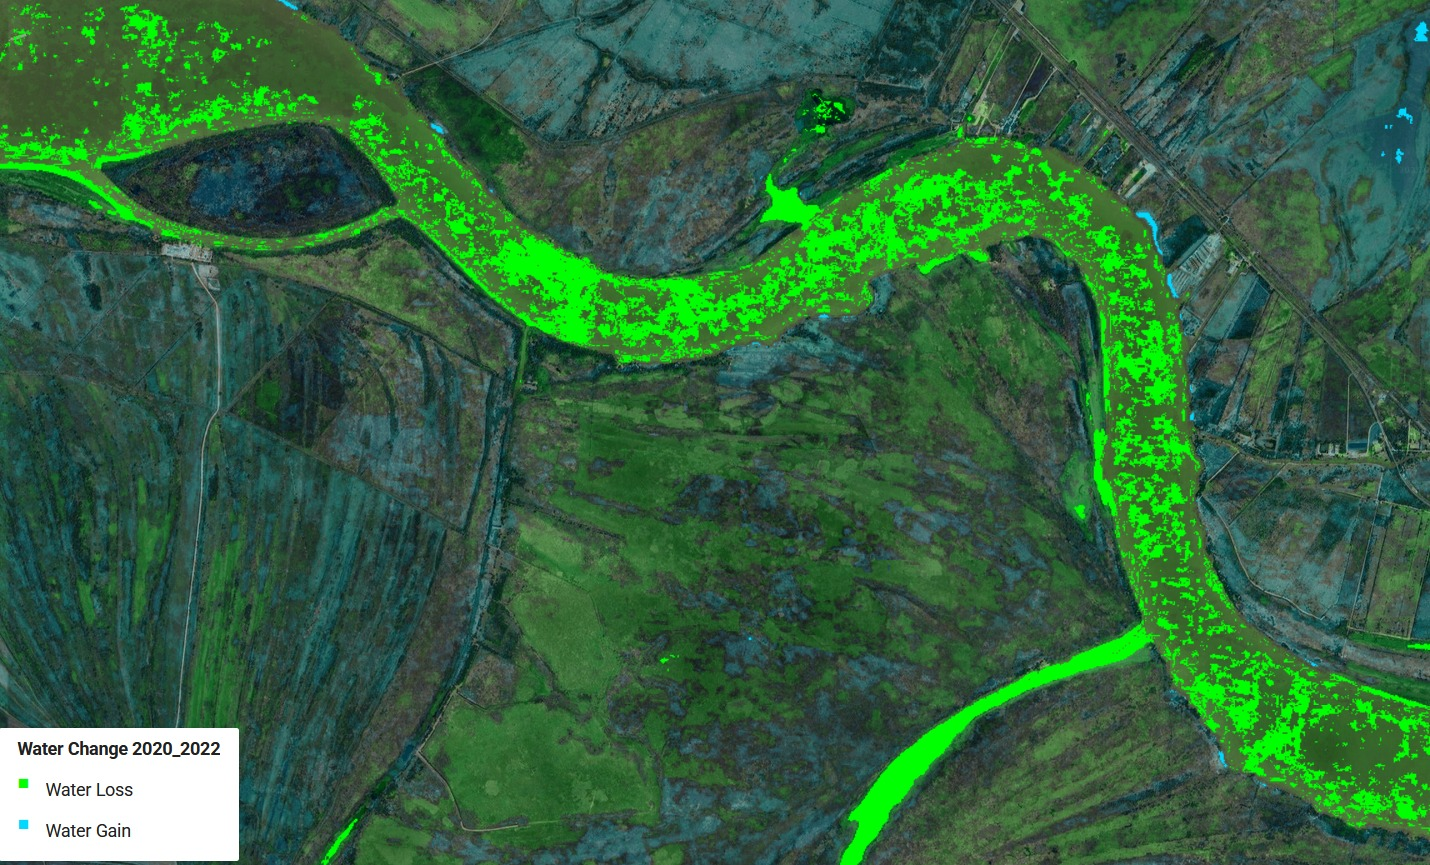
\includegraphics[width=\linewidth, height=5cm]{figures/ch5/2020-2022.jpg}
        \caption{Period 2020-2022}
        \label{fig:sontek}
    \end{subfigure}
    
    \caption{Water Changes in Different Periods}
    \label{fig:Water Changes}
\end{figure}

\begin{figure}[H]
    \centering
    \begin{subfigure}{0.6\textwidth}
        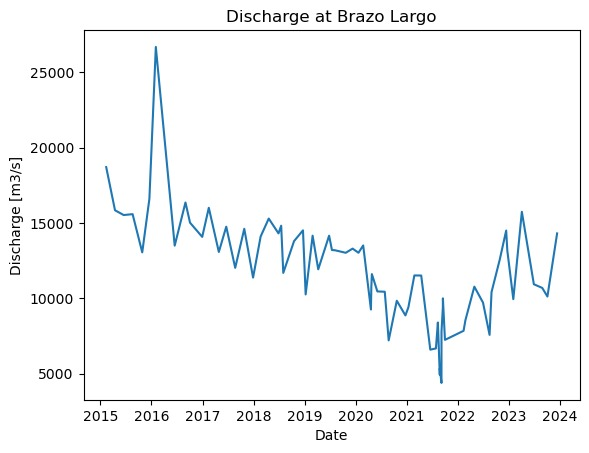
\includegraphics[width=\linewidth, height=5cm]{figures/ch5/dischargepeak.jpg}
    \end{subfigure}
    
    \caption{Discharge Changes in Brazo Largo}
    \label{fig:Discharge Changes in Brazo Largo}
\end{figure}


For the sake of these explanations the relevant Figures can be found in the Appendix \ref{Appendix: Satellite Data}.

\subsection{Surface Area Measurements}
From the Aqua Monitor Software, one could establish which regions were of interest in a broad scope surrounding the Parana Guazu turn near Puerto Constanza. 

Decreasing the scope leaves us with question marks regarding the actual areas and lengths of land that have been subject to these water gains. Therefore, it was chosen to investigate further into the details of the coast erosion with Google Earth.
Using the software's satellite data, one could draw a surface around the area of the Camping La Blanqueada in 2022, the most recent available, and then compare it to historical data. 
This gives a dataset of historical data from 1985 until 2022 but since the satellite images have been improving with the time, the only relevant data can be taken from 2003 on.


Thus, it was chosen to take the difference in surface area from 2022 until 2003. Initially only the East side of the Camping was taken into account due to its matching with the drone pictures taken of the area during the field trip \ref{fig:Bank Erosion shots from field work}. Nevertheless on Google Earth it quickly became obvious that the necessity rose to take the West part of the Camping in consideration as well since its surface was eroded even further.

A summary of the data gathered from this study can be found below. First the Measurement of the East part of the Camping, then the comparison with 2003, 2017, 2018 and then for both sides the added surface lost since 2003.

\begin{figure}[H]
    \centering
    \begin{subfigure}[b]{0.45\textwidth} % Adjusted width to fit both images side by side
        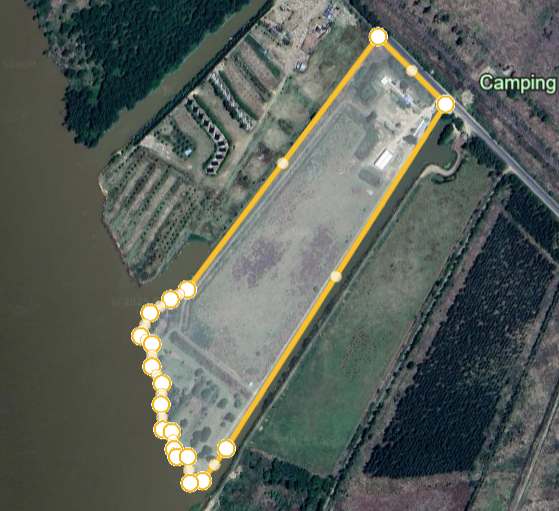
\includegraphics[width=\linewidth, height=5cm]{figures/appendix-g/opp2022.png}
        \caption{Surface Data for 2022}
        \label{fig:surface2022}
    \end{subfigure}
    \hfill
    \begin{subfigure}[b]{0.45\textwidth} % Adjusted width to fit both images side by side
        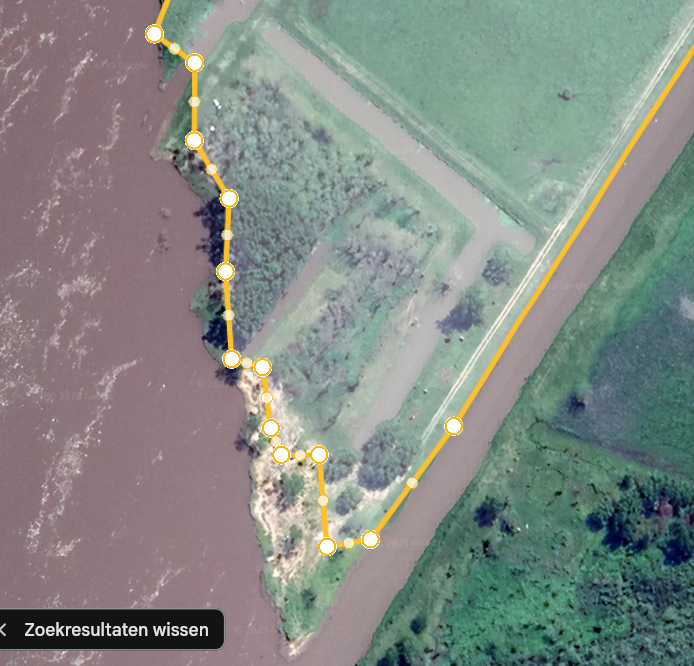
\includegraphics[width=\linewidth, height=5cm]{figures/appendix-g/opp2017.png}
        \caption{Surface Data for 2017}
        \label{fig:surface2017}
    \end{subfigure}
    \hfill
    \begin{subfigure}[b]{0.45\textwidth} % Adjusted width to fit both images side by side
        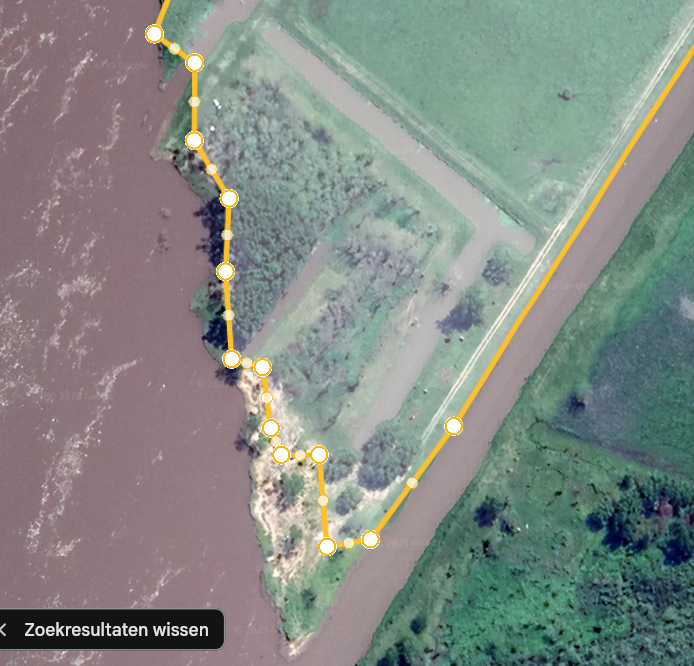
\includegraphics[width=\linewidth, height=5cm]{figures/appendix-g/opp2018.png}
        \caption{Surface Data for 2018}
        \label{fig:surface2018}
    \end{subfigure}
    \hfill
    \begin{subfigure}[b]{0.45\textwidth} % Adjusted width to fit both images side by side
        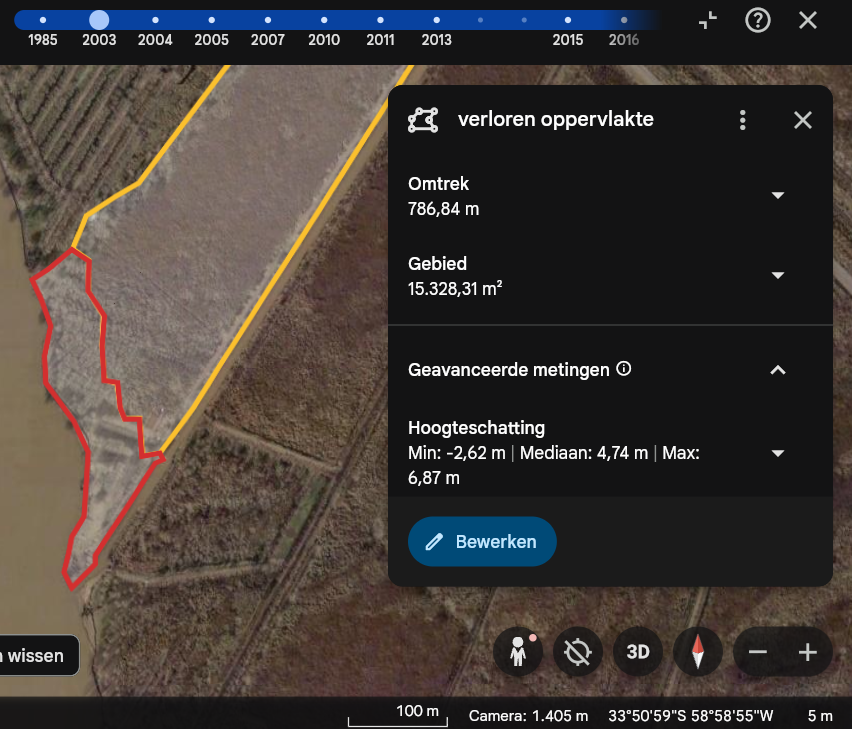
\includegraphics[width=\linewidth, height=5cm]{figures/appendix-g/verlorenopp2003.png}
        \caption{Surface Data for 2003}
        \label{fig:surface2003}
    \end{subfigure}
    \caption{Comparison of Surface Data}
    \label{fig:surface_comparison}
\end{figure}

It is known that there was a flood in 2016 \autocite{Inundacion}. This flood was in return responsible for a significant increase of water quantity and discharge throughout the region, as seen in Figure \ref{fig:Discharge Changes in Brazo Largo}.

Consequently this affected certain areas of the channel more than others, in particular the curves of the Parana Guazu such as Puerto Guazu showed in the Figures \ref{fig:Water Changes} as discussed before. The negative impacts were highlighted when the high discharge and water quantities dropped back to normal, leaving a part of the bank fragile which then contributed to an accelerated bank erosion.



This argument can once again be solidified by the drastic increase of erosion in between those time periods. After this flood event, the rate of erosion decreased again.

Lastly, both sides of the Camping and the difference between 2003 and 2022 can be seen below. The leftover piece of land which was present in 2003 but has been eroded since then is also traced as a surface area in a distinct colour \ref{fig:surfacelost_comparison}. 

\begin{figure}[H]
    \centering
    \begin{subfigure}[b]{0.45\textwidth} % Adjusted width to fit both images side by side
        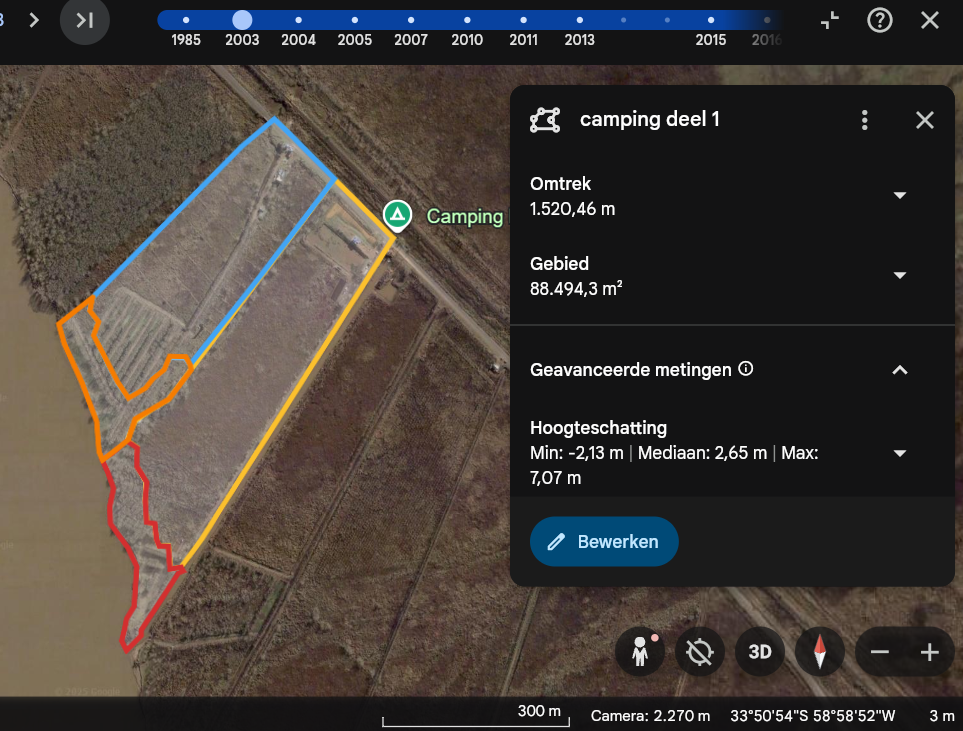
\includegraphics[width=\linewidth, height=5cm]{figures/appendix-g/delen2003.png}
        \caption{Surface Data for 2003}
        \label{fig:surface2003}
    \end{subfigure}
    \hfill
    \begin{subfigure}[b]{0.45\textwidth} % Adjusted width to fit both images side by side
        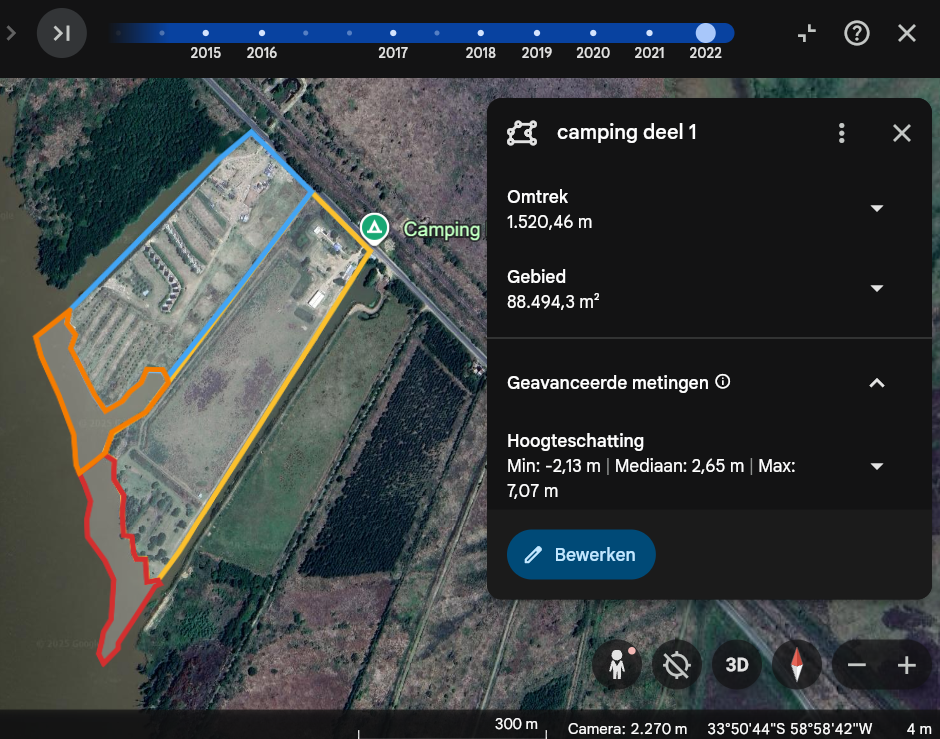
\includegraphics[width=\linewidth, height=5cm]{figures/appendix-g/delen2022.png}
        \caption{Surface Data for 2022}
        \label{fig:surface2022}
    \end{subfigure}
    \caption{Comparison of Lost Surface Data}
    \label{fig:surfacelost_comparison}
\end{figure}


The complete comparison with all accessible historical data was documented in the Appendix \ref{Appendix: Satellite Data}.

Moreover, values of the surface areas, perimeters, and further quantification's can be found in the next subsection.

\subsection{Quantitative Results}

The values of these areas can be found in the Table \ref{Table: Surface Recap Camping La Blanqueada in 2022}.

\begin{table}[h]
\centering
\caption{Surface Recap Camping La Blanqueada in 2022}
\label{tab:Surface Lost Camping La Blanqueada in 2022}
\begin{tabular}{l l l S[table-format=5.2] S[table-format=5.2]}
\toprule
\textbf{Location} & \textbf{Category} & \textbf{Colour} & \textbf{Perimeter (m)} & \textbf{Area (m²)} \\
\midrule
East Part & Actual & Yellow & 1520.46 & 88494.3 \\
East Part & Lost & Red & 786.84 & 15328.31 \\
West Part & Actual & Blue & 1203.31 & 71231.39 \\
West Part & Lost & Orange & 815.58 & 16179.99 \\
\bottomrule
\label{Table: Surface Recap Camping La Blanqueada in 2022}
\end{tabular}
\end{table}

From the values in Table G.2, one can calculate the rate of change in the last 20 years or so with the help of the following formula.

$\text{Loss Ratio} = \frac{\text{Loss}}{\text{Total Surface}}$

Consequently:

$\text{Loss Ratio} = \frac{\text{Loss}}{\text{Surface in 2022 + Loss}}$

Applying this to both sides of the Camping gives:

$\text{Loss Ratio (East)} = \frac{15328.31}{88494.3 + 15328.31}$
$=$ $\frac{15328.31}{103822.61} = 0.1476$ 

$\text{Loss Ratio (West)} = \frac{16179.99}{71231.39 + 16179.99}$ $=$
$\frac{16179.99}{87411.38} = 0.1851 $ 

Together, these results can are found in the Table \ref{Table:Loss Ratio for Camping La Blanqueada in 2022} .

\begin{table}[h]
\centering
\caption{Loss Ratio for Camping La Blanqueada in 2022}
\label{tab:LossRatio}
\begin{tabular}{l c}
\toprule
\textbf{Location} & \textbf{Loss Ratio (\%)} \\
\midrule
East Part & 14.76 \\
West Part & 18.51 \\
\bottomrule
\label{Table:Loss Ratio for Camping La Blanqueada in 2022}
\end{tabular}
\end{table}


\subsection{Qualitative Results}
From the quantitative results one can conclude that in 20 years there was a loss ratio of almost 15 to 18.5 \%. A qualitative approach gives an interesting point of view that is not based purely on numbers.

First of all, it is important to ask where these \% come from and what factor or problem contributes the most to the calculated erosion. We started from a quite biased point of view, the stakeholders. They told us that the reason for this erosion was purely the dredging of the sand and the cargo ships passing by. 

From the Wave impact study it shows that the cargo ships induced waves do in fact contribute to the bank erosion when passing by. It is quite hard to determine how much faster the erosion is happening due to this event but one might assume the fact that the contribution to the problem is small, but not insignificant. 


The Aqua Monitor study illustrates the high correlation between the water levels and discharge intensities with the water quantities gained in certain areas. The borders of curves in a channel are the most likely to be victim of the water gains which makes the bank stability decrease when the hydro parameters discharge and water quantity are restored to a normal level. This is as explained in the section \ref{}




-erosion due to natural climate?
-accelerated due to flooding the most. 
-waves of the ships contribute a bit still (from mike maybe?)
-worst factor is climate change. example of flood 2018 eroded soo much more than the boats. 